\chapter{Testing and Evaluation}
\label{chap:eval}
\lhead{\emph{Project Testing}}
%The goal of this chapter is an objective evaluation of the final system. The evaluation must be quantitative and not qualitative. You may perform qualitative evaluation but this should not form the basis of the main conclusions you derive from the evaluation. This evaluation, where possible, should be comparative, i.e. you should evaluate your system against a commercially available system and/or system detailed in a research publication. You should demonstrate operational testing of the project using real or contrived data sets to evaluate aspects of the project not encompassed in the software testing (e.g. quantify how well does your project achieved the overall goal). 
%\begin{itemize}
%    \item For software based projects this will include, but should not be limited to, evaluation of non-functional requirements.
%    \item For infrastructural projects this testing should include system/network KPI analysis.
%    \item For analysis based projects (ML, malware or other) this may include model evaluation or YARA rule validation, for example.
%    \item For management projects, where software testing or infrastructure testing may not be in scope, the test process for the system is expected to be more rigorous and well described than a project incorporating significant development work.
%\end{itemize} 
%
%Some suggested sections (the nature of this chapter should be discussed in detail with your term 2 supervisor):
%
%\section{Metrics}
%Identify and describe the metrics you used to evaluate your project. You should have identified some of these in the research phase report but will detail these as you progress through the design.
%
%\section{System Testing}
%Describe the experimental setup for each metric, and how you obtained the measurements. Describe the inputs for each experiment
%
%\section{Results}
%Summarise the output data, and the statistical or other techniques to deduce your results. Summarise your results, including tables or graphs as appropriate with a brief description of each. here possible, compare your results with other products/systems. Identify any possible threats to the validity of your results, and discuss each briefly here (you will discuss in more detail in the next chapter).
%
This chapter will go into more detail into how DynamiCrypt actually works. There will various code snippets present throughout this chapter. After an explanation of how parts of the system work tests will also be carried out. 

\section{The Beginning}
C++ is a compiled language and DynamiCrypt requires quite a few libraries to be present for linking. The command to compile DynamiCrypt is the following.
\begin{lstlisting}
g++ *.cpp -lboost_system -lpthread -lboost_thread -lboost_program_options -lcryptopp -lpistache -o DynamiCrypt
\end{lstlisting}

\begin{figure}[!h]
  \centering
      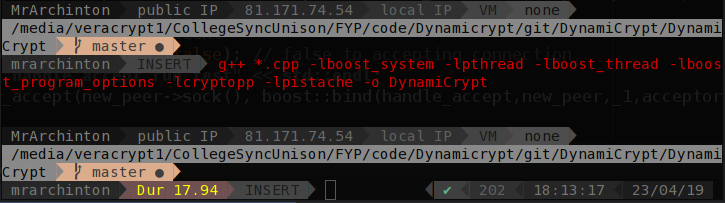
\includegraphics[width=1\textwidth]{Figures/b1.png}
  \caption[Compiling DynamiCrypt]{Compiling DynamiCrypt}
  \label{fig:b1}
\end{figure}
\FloatBarrier

Figure \ref{fig:b1} shows the result of the compilation and as you can see there are no errors or warnings present, this is an indication that the code is syntax correct and operations are performed for the correct data types.

Every program starts of with a main function. DynamiCrypt's main function is rather light, all it does is processes the command line arguments, creates a listening peer and creates the API server object.
To create an initial peer the already seen before code is used.
\begin{lstlisting}
ip::tcp::acceptor acceptor(service, ip::tcp::endpoint(ip::tcp::v4(), listen_port));
peer::ptr initial_peer = peer::new_(false);
acceptor.async_accept(initial_peer->sock(), boost::bind(handle_accept,initial_peer,_1, &acceptor));
\end{lstlisting}
Here an acceptor object is created this allows for the peer object to listen on a port on the localhost.
\begin{lstlisting}
peer::new_(false);
\end{lstlisting}
Is used to notify the peer object that this peer will be waiting for a connection.
\begin{lstlisting}
void handle_accept(peer::ptr peer, const boost::system::error_code & err, ip::tcp::acceptor* acceptor) {
    peer->start("",""); // starts current client
    // creates and listens for new client
    peer::ptr new_peer = peer::new_(false); // false to accepting connection
    //std::cout << "handle_accept run test" << std::endl;
    acceptor->async_accept(new_peer->sock(), boost::bind(handle_accept,new_peer,_1,acceptor)); // this 
}
\end{lstlisting}
The above function is called when the asynchronous connect object receives an external tcp request. The start method is called on the current peer followed by a creation of a new peer which will start listening for the next connection. This way there is always only one peer waiting for new connections. 

Because of how Boost manages asynchronous programming by using a service object to manage threads as well as using the proactor design pattern where asynchronous operations can occur using only one thread. However because DynamiCrypt is operation heavy when it comes to synchronisation I have used both threads and the proactor approach, this way when an asynchronous operation is about to take place Boost will choose a random available thread for it to run on. 
For this reason there are a few operations taking place in the main.cpp file to set all of this up.
\begin{lstlisting}
boost::thread_group threads;

start_listen(4);

void start_listen(int thread_count) {
    for ( int i = 0; i < thread_count; ++i)
        threads.create_thread( listen_thread);
}

void listen_thread() {
    service.run();
}

}
\end{lstlisting}
A group of threads variable is allocated, then the start listen function is called in the main function, this function creates four threads in this case and executes the service.run() function in each thread. This just executes boost asynchronous handler on each of the four threads. 

Finally to ensure a clean exit without leaving any zombie processes the main function will wait for all the threads to finish their execution.
\begin{lstlisting}
threads.join_all();
\end{lstlisting}

The API server is a bit more straight forward since the threads and asynchronous operations are more hidden away from the user by the Pistache library. 
\begin{lstlisting}
api_service_data_handler.set_address_and_port_of_sync("127.0.0.1", listen_port);
APIServer api_server(api_port);
\end{lstlisting}
The first line here sets the address of the sync-server and the port on which it is listening on as this information will be shared with the NodeJs app later. 
The actual creation of the API is simply calling the constructor with a port number.

The API and the sync-server require each other for operation, however it would be confusing if both were explained at the same time therefore the API will be covered initially followed by the sync-server.

\section{API}
The constructor of the API server creates the variables needed for the server and ofloads it to the APIservice object.
\begin{lstlisting}
APIServer::APIServer(int port_number) {
    Pistache::Port port(port_number);
    int thr = 2;
    Pistache::Address addr(Pistache::Ipv4::any(), port);
    //cout << "Cores = " << hardware_concurrency() << endl;
    std::cout << "API Using " << thr << " threads" << std::endl;
    API_service api(addr);
    api.init(thr);
    api.start();
    api.shutdown();
}
\end{lstlisting}
For the API two threads were defined as this is enough to handle multiple clients.
The threads are created as follows.
\begin{lstlisting}
void API_service::init(size_t thr = 2) {
    auto opts = Pistache::Http::Endpoint::options()
        .threads(thr)
        .flags(Pistache::Tcp::Options::InstallSignalHandler);
    httpEndpoint->init(opts);
    createDescription();
}
\end{lstlisting}
Pistache is a much more high level library than Boost therefore for the setup I mostly followed the examples they have in their GitHub repository.
\begin{lstlisting}
void API_service::start() {
    router.initFromDescription(desc);
    httpEndpoint->setHandler(router.handler());
    httpEndpoint->serve();
}
\end{lstlisting}
start() sets up the description which in Pistache's case is the information about all the routes available, some licensing and API info.  

Here is a small extract from the function that creates the description
\begin{lstlisting}
void API_service::createDescription() {
    desc
        .info()
        .license("Apache", "http://www.apache.org/licenses/LICENSE-2.0");

    auto backendErrorResponse =
        desc.response(Pistache::Http::Code::Internal_Server_Error, "An error occured with the backend");

    desc
        .schemes(Pistache::Rest::Scheme::Http)
        .basePath("/v1")
        .produces(MIME(Application, Json))
        .consumes(MIME(Application, Json));

    auto versionPath = desc.path("/v1");

    auto path = versionPath.path("/options");

    path
        .route(desc.get("/test-ok"))
        .bind(&API_service::route_test, this)
        .produces(MIME(Application, Json), MIME(Application, Xml))
        .response(Pistache::Http::Code::Ok, "ok");
    
    path
        .route(desc.post("/init"), "Initiate Communication")
        .bind(&API_service::initial, this)
        .produces(MIME(Application, Json))
        .consumes(MIME(Application, Json))
        .response(Pistache::Http::Code::Ok, "Initial request")
        .response(backendErrorResponse);
\end{lstlisting}
The path is built by firstly specifying the version of the API this way it is possible to support legacy code using you old API. Next I decided to put all the DynamiCrypt operations preceded by /options this way in the future if the API can be expanded to do other things like maybe formatting / encoding data. Next is the actual routes used by the DynamiCrypt API. The first one is /test-ok a GET route, this is handy if you want to check if the API is up and running. To access this route you would send a get request to this for example 127.0.0.1:9081/v1/options/test-ok/. This simple route will just return "ok" as can be seen when a curl get request is being made as can be seen in figure \ref{fig:b2}.

\begin{figure}[!h]
  \centering
      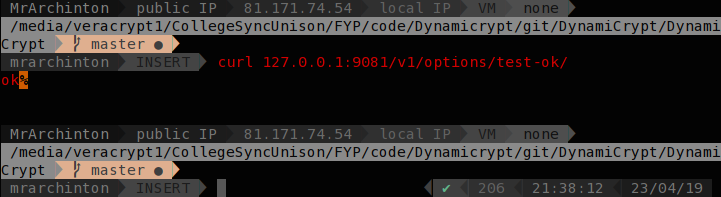
\includegraphics[width=1\textwidth]{Figures/b2.png}
  \caption[127.0.0.1:9081/v1/options/test-ok/]{127.0.0.1:9081/v1/options/test-ok/}
  \label{fig:b2}
\end{figure}
\FloatBarrier

The list of all routes currently available in the API and a brief description are as follows.
\begin{lstlisting}
/v1/options/test-ok         GET
// test if API is up
/v1/options/init            POST
// Initial request
/v1/options/init_config     POST
// Initial Config
/v1/options/sync            POST
// Begin Sync
/v1/options/status          POST
// check if connected to tpm ok
/v1/options/encrypt         POST
// encrypt / decrypt data
/v1/options/exit            POST
// delete tpm and data associated with the app using the API
/v1/options/:rest           POST
// custom 404
\end{lstlisting}

Every post route is handled by a specific function.
\begin{lstlisting}
 path
        .route(desc.post("/init"), "Initiate Communication")
        .bind(&API_service::initial, this)
        .produces(MIME(Application, Json))
        .consumes(MIME(Application, Json))
        .response(Pistache::Http::Code::Ok, "Initial request")
        .response(backendErrorResponse);
\end{lstlisting}

In this case every time the init route is called the initial() function handles it and produces its own response. Here is the initial function bellow.

\begin{lstlisting}
void API_service::initial(const Pistache::Rest::Request& request, Pistache::Http::ResponseWriter response) {
    rapidjson::Document document;
    // make into json object
    char * jsonBody = new char [request.body().length()+1];
    strcpy (jsonBody, request.body().c_str());
    document.Parse(jsonBody);
    
    std::string service_name;
    int data_ok = 1;

    if(document.HasMember("service_name")){
        if(document["service_name"].IsString()){
            service_name = document["service_name"].GetString();
        }
        else{
            data_ok = 0;
        }
    }
    else{
        data_ok = 0;
    }
    
    std::string respond_service_name;
    rapidjson::StringBuffer buffera;
    rapidjson::Writer<rapidjson::StringBuffer> writera(buffera);
    
    if(data_ok){
        respond_service_name = api_service_data_handler.new_service(service_name);
        writera.StartObject(); 
        writera.Key("service_name");                
        writera.String(respond_service_name.c_str(), respond_service_name.length());
        writera.Key("address_of_this_tpm");                
        writera.String(api_service_data_handler.get_sync_address().c_str(), api_service_data_handler.get_sync_address().length());
        writera.Key("port_of_this_tpm");
        writera.Uint(api_service_data_handler.get_sync_port());
        writera.EndObject();
        
    }
    
    else{//error with request
        writera.StartObject(); 
        writera.Key("error");                
        writera.String("invalid request");
        writera.EndObject();
    }
    
    response.send(Pistache::Http::Code::Ok, buffera.GetString());
}
\end{lstlisting}

Similar to NodeJs each of these handlers have a reference to a request and response object.
For extracting JSON data the RapidJson library is used, it is also used for creating JSON data.
The API interacts with the 
\begin{lstlisting}
api_service_data_handler
\end{lstlisting} 
object for managing the services.

It will take too long to go through all of the routes and how they function so a more basic explanation will suffice. I would recommend watching my demo video here https://www.youtube.com/watch?v=LsR4XsGrDCY&feature=youtu.be 
on YouTube as it would be easier to understand.

Initially the NodeJs apps must register with the API this unfortunately turned out to be a multi step process however it is necessary since the API needs data from both of the Apps that wish to use DynamiCrypt.

\begin{figure}[!h]
  \centering
      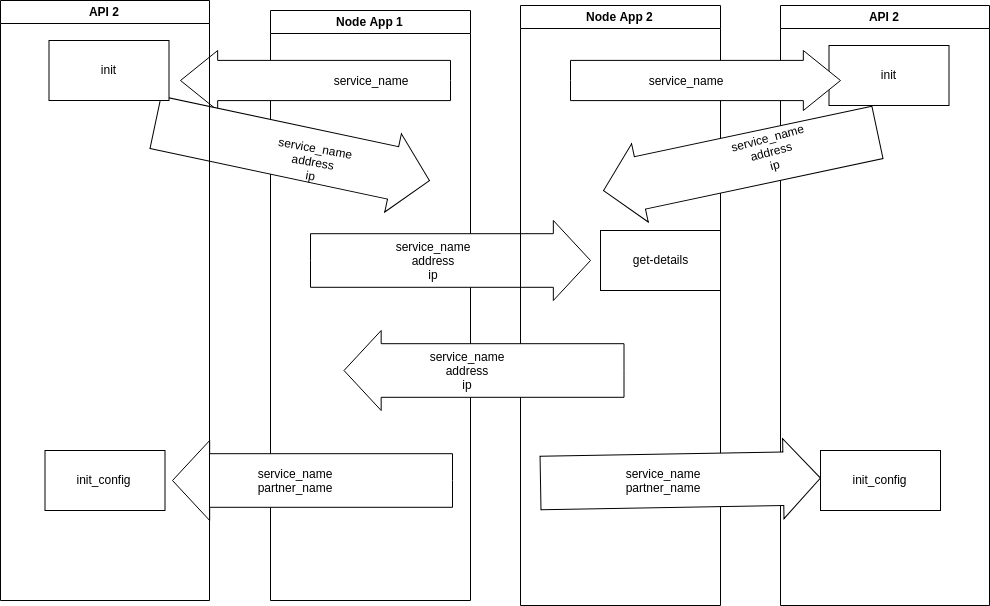
\includegraphics[width=1\textwidth]{Figures/connect_code_flow.png}
  \caption[How Node Apps register with the API]{How Node Apps register with the API}
  \label{fig:b3}
\end{figure}
\FloatBarrier

Figure \ref{fig:b3} is a call flow diagram of how the NodeJS apps register themselves with the API.
The same can be demonstrated by using Wireshark and listening on localhost. The filters I used are (tcp.port == 9081) && http since I only want to see POST requests for the API running on port 9081 since the POST requests for the other API are identical so there is no point in showing it twice.

\begin{figure}[!h]
  \centering
      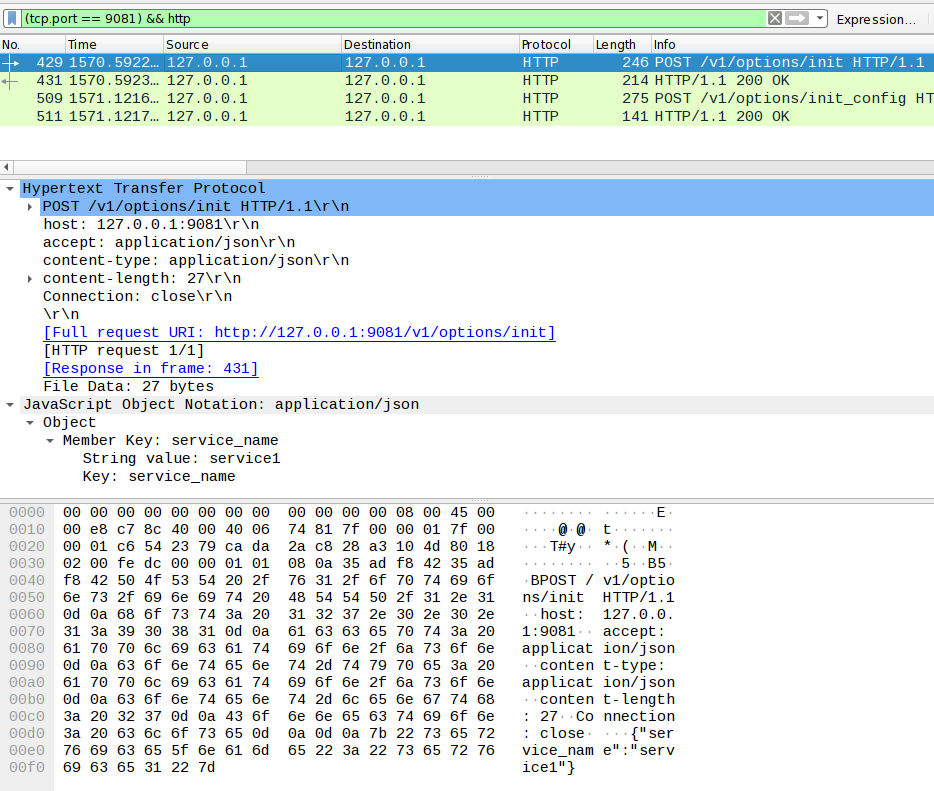
\includegraphics[width=1\textwidth]{Figures/b4.png}
  \caption[POST request to init]{POST request to init}
  \label{fig:b4}
\end{figure}
\FloatBarrier
Figure \ref{fig:b4} shows how the NodeJs App sent a POST request to the init route with its user service name. 

\begin{figure}[!h]
  \centering
      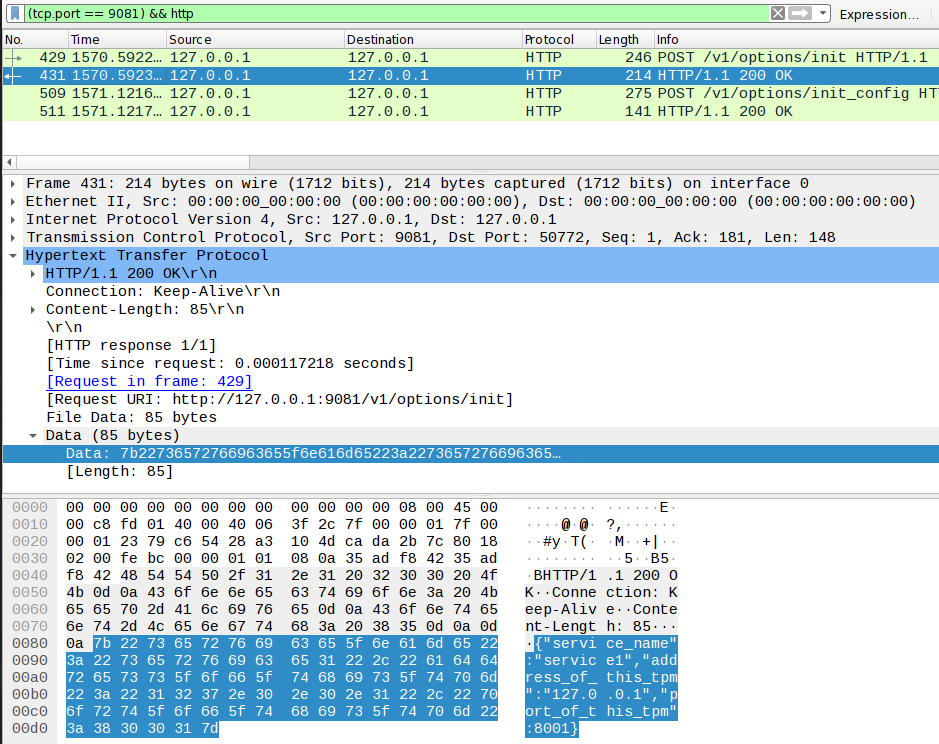
\includegraphics[width=1\textwidth]{Figures/b5.png}
  \caption[API response]{API response}
  \label{fig:b5}
\end{figure}
\FloatBarrier
Figure \ref{fig:b5} shows how the APIs reply to the previous post request with the service name the API wants the NodeJS App to use, the port of the sync-server and the address of the sync-server.
After this the Node App would make a request to the other Node App for the get details route to exchange information. This can also be acquired with Wireshark by changing a filter as seen in figure \ref{fig:b8}.
\begin{figure}[!h]
  \centering
      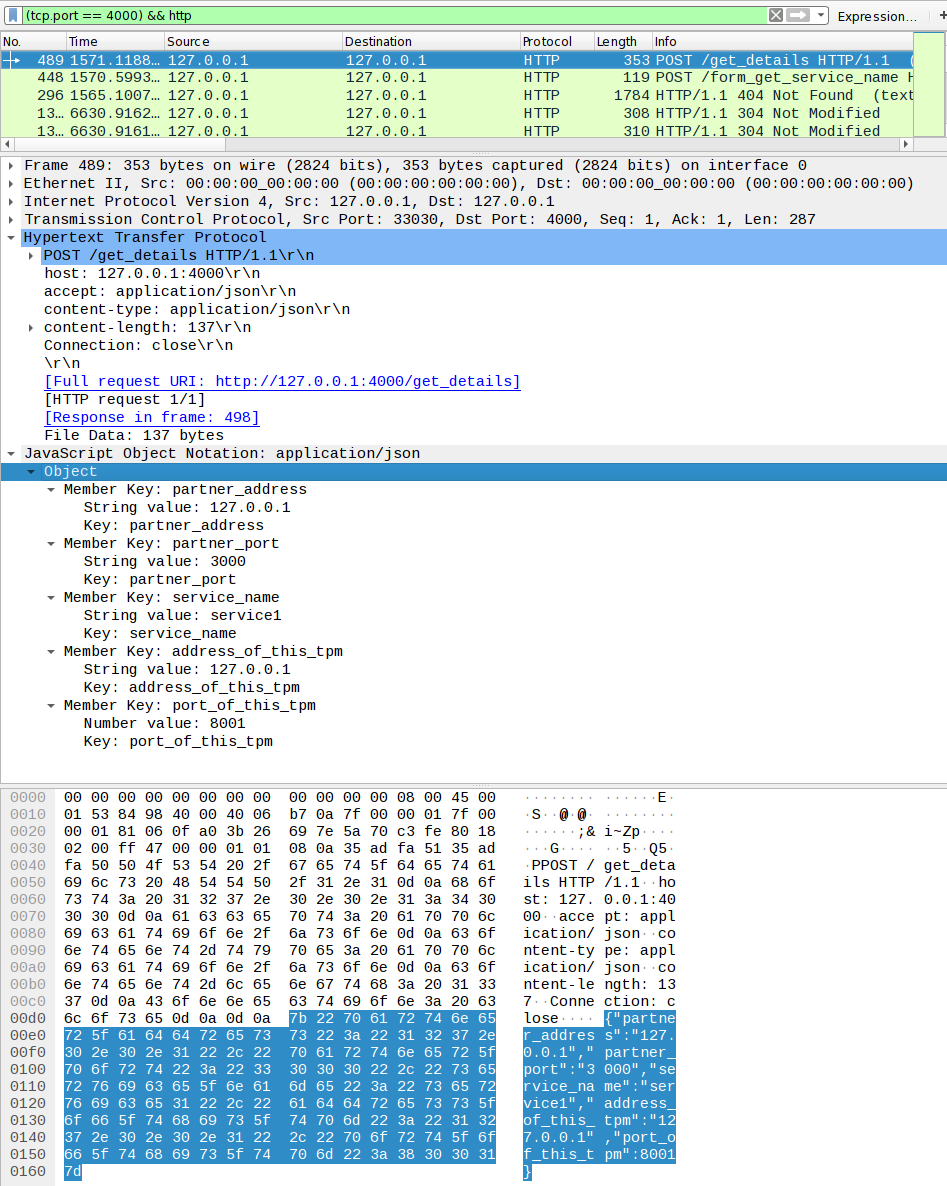
\includegraphics[width=1\textwidth]{Figures/b8.png}
  \caption[POST request to other NodeJs app's get details route]{POST request to other NodeJs app's get details route}
  \label{fig:b8}
\end{figure}
\FloatBarrier


\begin{figure}[!h]
  \centering
      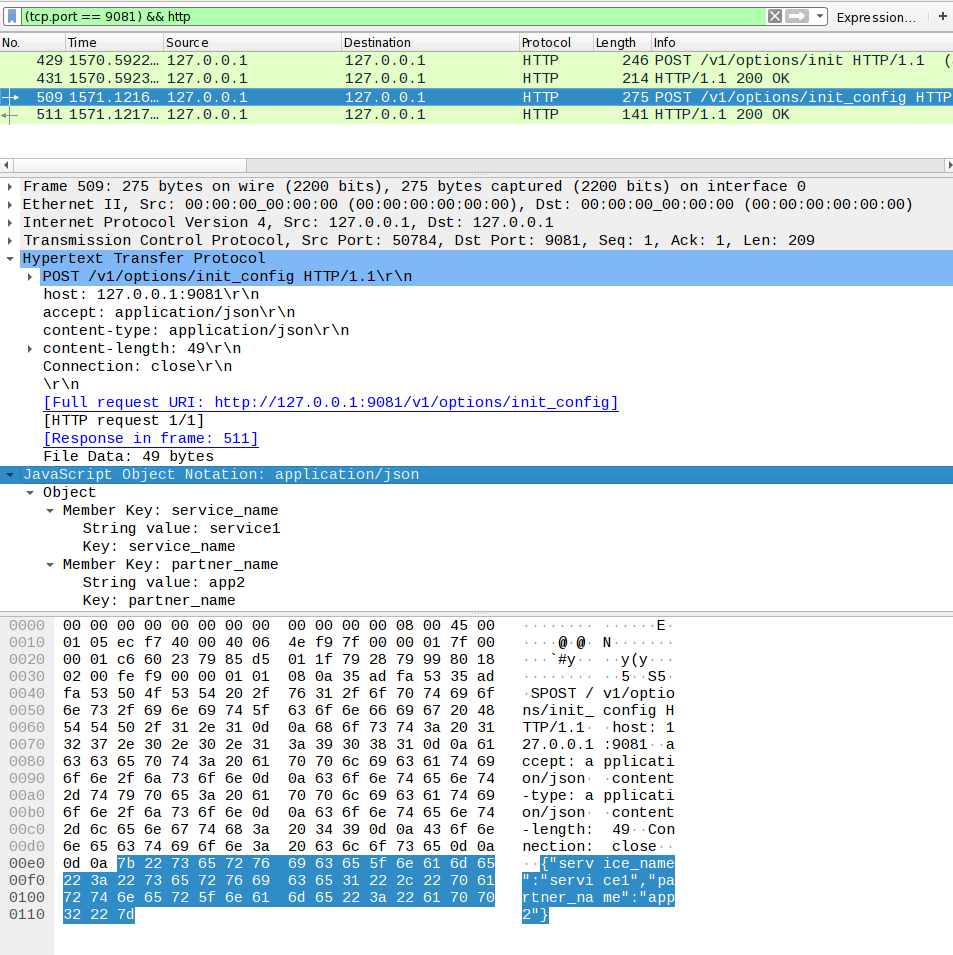
\includegraphics[width=1\textwidth]{Figures/b6.png}
  \caption[POST request to init config]{POST request to init config}
  \label{fig:b6}
\end{figure}
\FloatBarrier
Figure \ref{fig:b6} shows how the NodeJs app updates the API with the service name of the other NodeJs app in this case it is called partner name.

\begin{figure}[!h]
  \centering
      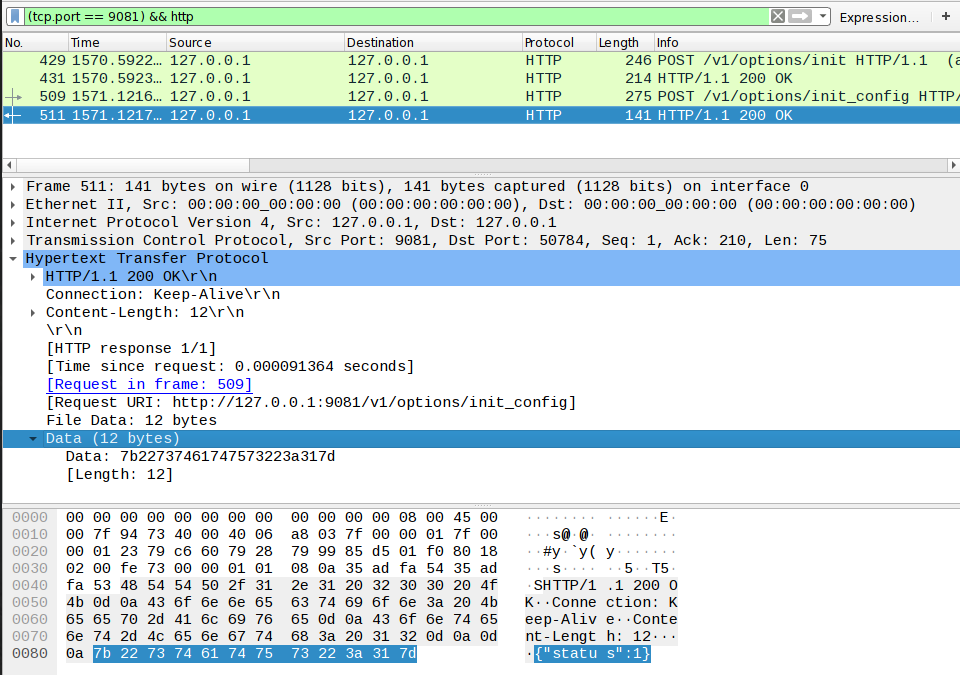
\includegraphics[width=1\textwidth]{Figures/b7.png}
  \caption[API response]{API response}
  \label{fig:b7}
\end{figure}
\FloatBarrier
Figure \ref{fig:b7} shows the APIs reply to the previous post request with a status 1 which means everything is OK and the update was successfully made.
Now the two NodeJs apps are fully registered with the API. The next step is to tell the API to tell the sync-server to start synchronising so that the Apps can send messages to each other using dynamic encryption.
For this to occur one of the Apps must simply call the sync route of the API.

\begin{figure}[!h]
  \centering
      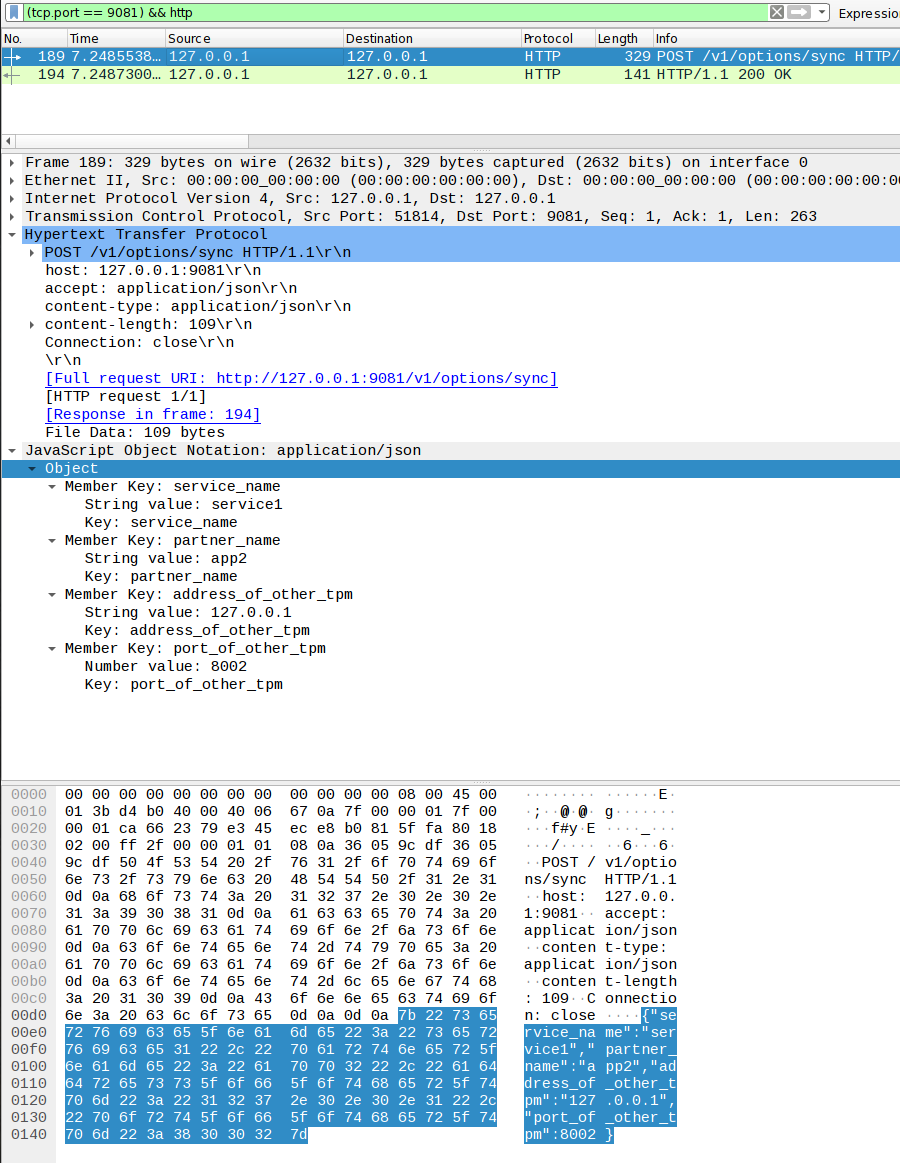
\includegraphics[width=1\textwidth]{Figures/b9.png}
  \caption[POST request to sync]{POST request to sync}
  \label{fig:b9}
\end{figure}
\FloatBarrier
Figure \ref{fig:b9} shows the sync route of the API is called. The Node App sends a lot of details this time including service name, partner name, the address and port of the sync-server that is used by the other API that the other NodeJs App communicates with. This is because it is calling a different function outside of the api service data handler object. This time a function from the definitions.cpp is called.
\begin{lstlisting}
int begin_sync(std::string address, int port, std::string service_name, std::string partner_name){
    try{
        peer::ptr initiating_peer = peer::new_(true, address, port);
        initiating_peer->start(service_name, partner_name);
    }
    catch(std::exception& e){
        return 0;
    }
    return 1;
}
\end{lstlisting} 
Here a new peer is created of connecting type instead of listening type like we looked at last time. This peer will try to connect to the sync-server at the address and port the Node App sent it.

\begin{figure}[!h]
  \centering
      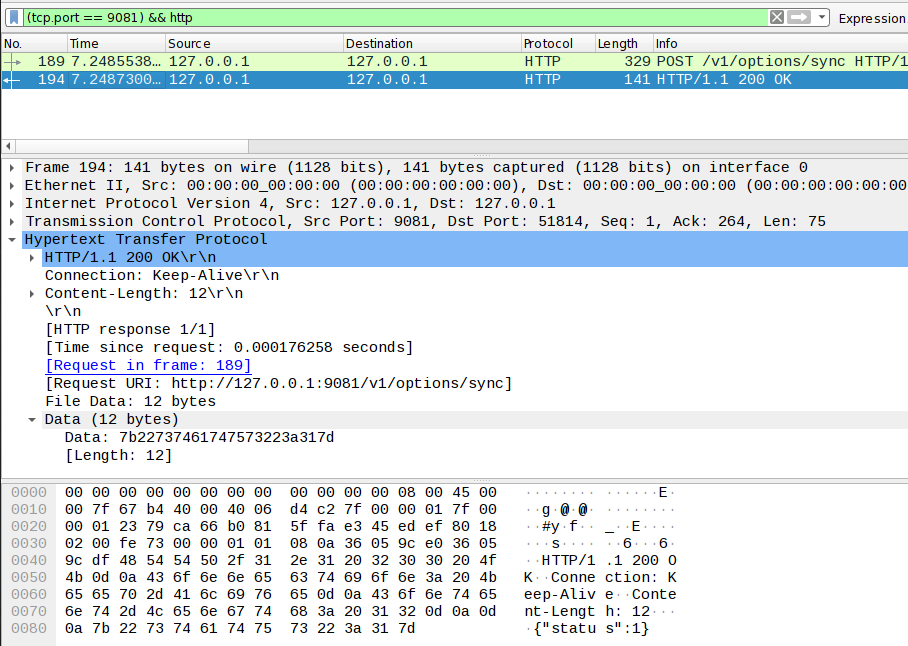
\includegraphics[width=1\textwidth]{Figures/b10.png}
  \caption[API response]{API response}
  \label{fig:b10}
\end{figure}
\FloatBarrier
Figure \ref{fig:b10} shows the APIs reply to the previous post request with a status 1 which means the request was processed successfully however this does not mean that the sync-server connected to the other sync-server correctly this is because of the asynchronous nature of the sync-server it is impossible to get the result of the connection. Therefore the NodeJs app should query the API to see if the connection was successful and if the two sync-servers are currently syncing this is done by calling the status route in the API and providing the service name. if the status returned is 1 then the two sync-servers are currently synchronising, if the status is 0 then they failed to connect or some other error occurred.

\textbf{Encryption / Decryption}

Now the NodeJs apps can send messages to the API to be encrypted.
How encryption works is it selects the appropriate key from the key store based on the mode provided.
The key store looks like this.
\begin{lstlisting}
struct key_store {
    std::string key;
    int uses;
};

struct API_data {
    std::string service_name_;
    std::string service_name_partner_;
    std::vector<key_store> keys_;
};
\end{lstlisting} 
This is an inner struct inside the 
\begin{lstlisting}
API_service_data_handler
\end{lstlisting} 
class which contains a vector of API data objects.

Currently DynamiCrypt supports two encryption methods. Encryption mode 1 will simply use the latest key avaiable in the keystore, this mode is handy if you want the fastest mode of encryption available.
For encryption mode 1, 
\begin{lstlisting}
if(mode == 1){
                //check for any latest key 
                if(api_data->keys_.size() == 0){
                    return DYNAMICRYPT_API_WAIT;
                }else{
                    string_key = api_data->keys_.back().key;
                    api_data->keys_.back().uses ++;
                    if(PRINT_API_CRYPT_MESSAGES){
                        std::cout << "got key like this " << string_key << std::endl;
                        std::cout << "key was used " << api_data->keys_.back().uses << " times" << std::endl;
                    }
                }
            
            }
\end{lstlisting} 
The appropriate api data object is selected referring to the service that called the API.
The size of the key store is initially checked to see if it contains any keys, if not then the API will tell the Node App to wait. The node app can then query the API again and again for encryption or just use a timeout and wait for 100 milliseconds or so. 
If there is keys in the key store then the last key that was entered is used for encryption. The uses count of this particular key is also increased, the uses count doesn't really matter for mode 1 but will matter for mode 2 and future modes that are not implemented yet. 

Encryption mode 2 would be the more secure one as only keys that have 0 uses are picked this way each message would be encrypted using its own unique key.
\begin{lstlisting}
else if (mode == 2){
                if(api_data->keys_.size() == 0){
                    return DYNAMICRYPT_API_WAIT;
                }
                else{
                    int attempts_to_find_key = 0; //search max_attempts_to_decrypt times for the key since decrypt will only search for max_attempts_to_decrypt times too
                    int found_key = 0;
                    for(int number_of_keys = api_data->keys_.size()-1; number_of_keys >= 0; number_of_keys --){
                        if(attempts_to_find_key == max_attempts_to_decrypt){
                            break;
                        }
                        attempts_to_find_key ++;
                        if(api_data->keys_.at(number_of_keys).uses == 0){
                            string_key = api_data->keys_.at(number_of_keys).key;
                            api_data->keys_.at(number_of_keys).uses++;
                            if(PRINT_API_CRYPT_MESSAGES){
                                std::cout << "got key like this " << string_key << std::endl;
                                std::cout << "key was used " << api_data->keys_.at(number_of_keys).uses << " times" << std::endl;
                            }
                            found_key = 1;
                            break;
                        }
                    }
                    if(!found_key){
                        return DYNAMICRYPT_API_WAIT;
                    }
                }
            }
\end{lstlisting} 
This mode is a little bit more involved then the simple get latest key. The Basic premise here is to find a suitable key that has 0 uses. This key is found by working back from the latest key down the vector until either a key is found, either the number of keys runs out or the search limit is reached. in this case the search limit is defined at 10 and stored at this variable.
\begin{lstlisting}
max_attempts_to_decrypt
\end{lstlisting} 
This means that in order to find a key provided the key store is longer than 10 the search will max out at 10 elements from the latest. 
This limit is set not so much for encryption but rather the decryption, this is because if there was no limit the encryption algorithm might choose a key that is say 200 keys away from the latest, the decryption algorithm will then have a heck of a time trying to find that correct key to use. 
And just like before if an appropriate key is not found the API will tell the Node App to wait.

After these two algorithms find the appropriate key the next step is to encrypt the data.
\begin{lstlisting}
CryptoPP::byte key[ CryptoPP::AES::MAX_KEYLENGTH ];
gen_key(string_key,key);
std::string for_encode = encrypt(message, key, iv);
\end{lstlisting} 
Earlier I said that the key generated by the tree parity machines will be used to encrypt the message. This is technically not true since that key is actually used to generate the actual key used for encryption. This is because the key generated by the tree parity machines is too long for AES-256 encryption therefore the gen key function generates an appropriate size key without loosing any data, this means that it does not simply cut of the rest of the key that's longer than 32 bytes needed for AES-256. Here is a snippet from that function.
\begin{lstlisting}
void API_service_data_handler::gen_key(std::string string_key, CryptoPP::byte* key){
    if(string_key.length() > CryptoPP::AES::MAX_KEYLENGTH){
            int count_first = 0;
            int count_last = string_key.length() -1;
            int number_of_operations = count_last - CryptoPP::AES::MAX_KEYLENGTH;
            for(int i = 0; i< number_of_operations; i++){
                string_key[count_first] = string_key.at(count_first) + string_key.at(count_last);
                if(count_first == CryptoPP::AES::MAX_KEYLENGTH){
                    count_first = 0;
                }
                count_first ++;
                count_last --;
            }
        }
        
        int string_count = 0;
        for(int i=0; i<CryptoPP::AES::MAX_KEYLENGTH; i++){
            if(string_count == string_key.length() -1){
                string_count = 0;
            }
            key[i] = string_key.at(string_count);
            string_count ++;
        } 
\end{lstlisting} 

After encrypting the data, the ciphertext is then encoded with base 64 encoding. Encoding is necessary because random bytes tend to mess up the structure of the JSON object.
\begin{lstlisting}
std::string encoded = encode_base64(for_encode);
output = encoded;
\end{lstlisting} 

Finally when sending the ciphertext to the node app the API also generates a hash specifically SHA 256 of the original plaintext. this will help the API to determine if the message was decrypted successfully by comparing hashes. Hashes are one way function so it is save to create a hash of the plaintext. The node app would then essentially just forward the ciphertext and the hash to the other node app for decrypting.

Decryption has algorithms specific for each mode therefore decryption mode 1 will directly be capable of decrypting encryption mode 1 and so on. The decryption is a potentially much more operation heavy operation that encryption. This is because it takes a guess at the key then tries to decrypt it and if that fails takes a guess at another key. This might seen pretty bad but from testing normally it only takes one to three decryption attempts to decrypt the key since the most likely key would be the latest one.

The decryption section of the code initially decodes the data from base 64 then that data is passed to the various decryption algorithms based on the mode.

For decryption mode 1
\begin{lstlisting}
if(mode == 1){
                if(api_data->keys_.size() == 0){
                    return DYNAMICRYPT_API_WAIT; // no keys in key ring shouldn't happen with decrypt if used properly
                }
                int number_of_keys = api_data->keys_.size()-1;  // maybe change to keys_.size()-1
                for(int decrypt_loop = 0; decrypt_loop<max_attempts_to_decrypt; decrypt_loop++){
                    //try last key first
                    std::string string_key = api_data->keys_.at(number_of_keys).key;
                    if(PRINT_API_CRYPT_MESSAGES){
                        std::cout << "trying to decrypt with key " << string_key << std::endl;
                        std::cout << "key was used " << api_data->keys_.at(number_of_keys).uses << " times" << std::endl;
                    }
                    CryptoPP::byte key[ CryptoPP::AES::MAX_KEYLENGTH ];
                    gen_key(string_key,key);

                    output = decrypt(decoded_message, key, iv);
                    if(!hash_with_sha_256(output).compare(hash)){ //decrypted successfully
                        api_data->keys_.at(number_of_keys).uses ++;
                        break;
                    }

                    if(number_of_keys == 0){
                        //output = "failed";
                        return DYNAMICRYPT_API_FAILED_DECRYPT;
                        break;
                    }

                    number_of_keys --;
                
                }
            }
\end{lstlisting} 
This checks if there are keys in the key ring this is not necessary since the tree parity machines generate the same keys at pretty much the same time but it is just in there as a sanity check or to catch some other strange errors. This is because for decryption the key is presumed to exist since that key was used to encrypt in the first place.

Since this is mode 1 we can simply try the latest key first then work down from there. Again how much further down you can go depends on the size of the key store and the limitation put in place to prevent traversing all the keys in case of an error or broken data.

Next the message is decrypted and hashed and the hash is compared to the hash sent by the node app. if the hashes match then the plaintext is returned if not the next key in line is tested.
If the hashes match the uses for the key is incremented this is important because you don't want this API using the same key for encryption as the other API if using mode 2. 
In the unlikely event that all the keys tried failed to decrypt the message a failure message will be sent to the node App, during testing I never have seen this scenario occur however it is likely to happen if you delay sending the encrypted data for decryption by quite some time like ten or more seconds since the key store will be filled up with new keys and the old key required for decryption will be pushed back past the limit. For this reason it is important for the node apps to send the ciphertext to the other node app as soon as possible.

For decrypting mode 2 quite a long algorithm is used. 
\begin{lstlisting}
else if (mode == 2){ // try keys with 0 uses first
                std::string string_key;
                if(api_data->keys_.size() == 0){
                    return DYNAMICRYPT_API_WAIT; // no keys in key ring shouldn't happen with decrypt if used properly
                }
                int has_skipped_keys = 0;
                int number_of_keys = api_data->keys_.size()-1;  // maybe change to keys_.size()-1
                
                //std::cout << "number_of_keys at start " << number_of_keys << std::endl;
                std::vector<int> skipped_keys;
                for(int decrypt_loop = 0; decrypt_loop<max_attempts_to_decrypt; decrypt_loop++){
                    //std::cout << "decrypt_loop at start " << decrypt_loop << std::endl;
                    if(number_of_keys == -1){ // needed because of the continue which could cause number_of_keys to be -1
                        break;
                    }
                    
                    if(api_data->keys_.at(number_of_keys).uses == 0){
                        
                        string_key = api_data->keys_.at(number_of_keys).key;
                        //std::cout << "key with 0 uses found " << string_key << std::endl;
                    }else{
                        skipped_keys.push_back(number_of_keys);
                        //std::cout << "skipping key at index " << number_of_keys << std::endl;
                        number_of_keys --;
                        has_skipped_keys = 1;
                        
                        continue;
                    }
                    
                    if(PRINT_API_CRYPT_MESSAGES){
                        std::cout << "trying to decrypt with key " << string_key << std::endl;
                        std::cout << "key was used " << api_data->keys_.at(number_of_keys).uses << " times" << std::endl;
                    }
                    CryptoPP::byte key[ CryptoPP::AES::MAX_KEYLENGTH ];
                    gen_key(string_key,key);

                    output = decrypt(decoded_message, key, iv);
                    if(!hash_with_sha_256(output).compare(hash)){ //decrypted successfully
                        api_data->keys_.at(number_of_keys).uses ++;
                        return output;
                    }

                    if(number_of_keys == 0){
                        break;
                    }

                    number_of_keys --;
                
                }
                //code runs here only if decryption was unsuccessful
                if(has_skipped_keys){ //check for skipped keys
                    for(int i = 0; i < skipped_keys.size(); i ++ ){
                        string_key = api_data->keys_.at(i).key;
                        if(PRINT_API_CRYPT_MESSAGES){
                            std::cout << "trying to decrypt with key " << string_key << std::endl;
                            std::cout << "key was used " << api_data->keys_.at(i).uses << " times" << std::endl;
                        }
                        CryptoPP::byte key[ CryptoPP::AES::MAX_KEYLENGTH ];
                        gen_key(string_key,key);

                        output = decrypt(decoded_message, key, iv);
                        if(!hash_with_sha_256(output).compare(hash)){ //decrypted successfully
                            api_data->keys_.at(i).uses ++;
                            return output;
                        }
                    }
                    // if key not decrypted then code is continued here therefore
                    //output = "failed";
                    return DYNAMICRYPT_API_FAILED_DECRYPT;
                }else{
                    //output = "failed";
                    return DYNAMICRYPT_API_FAILED_DECRYPT;
                }

            }
\end{lstlisting} 
The reason this is quite long is because of the introduction of skipped keys. Because for encryption mode 2 we only use a key with 0 uses. Therefore to speed up decryption we can test all the keys within the limit that have 0 uses since keys with 0 uses are most likely to decrypt the message for mode 2. 
If the keys with 0 uses fail to decrypt then the keys with more than 0 uses are that were skipped are tested, this should not happen but due to network latency it can be possible where both of the node apps send an encrypt request with mode 2 at the same time and the API manages to use the same key for both, this is very unlikely however just in case it does the code can take care of this scenario, and adding code here doesn't decrease the performance at all since it is just an if statement wouldn't even be called because of the break if the keys with 0 uses successfully decrypted the message. 

Now that we have an idea of how the encryption / decryption operates its time to demonstrate it in action.
I will use the quick setup python script to register the node apps quickly. The quick setup simply "fills out the forms" via code rather than hand. The script looks like this and is included in the Github repository.
\begin{lstlisting}
#!/usr/bin/env python3.7

import requests
import time

Service_one_name = "service1"
Service_two_name = "app2"

Service_one_address = "127.0.0.1"
Service_one_port = 3000

Service_two_address = "127.0.0.1"
Service_two_port = 4000

Service_one_API_address = "127.0.0.1"
Service_two_API_address = "127.0.0.1"

Service_one_API_port = 9081
Service_two_API_port = 9082


url1 = "http://" + Service_one_address + ":" + str(Service_one_port) + "/form_get_service_name"
data = {'Service_name':Service_one_name, 'API_port': Service_one_API_port, 'API_Address': Service_one_API_address} 

r = requests.post(url = url1, data = data) 


url1 = "http://" + Service_two_address + ":" + str(Service_two_port) + "/form_get_service_name"
data = {'Service_name':Service_two_name, 'API_port': Service_two_API_port, 'API_Address': Service_two_API_address} 

r = requests.post(url = url1, data = data) 

time.sleep(0.5)

# now send info to parnter
url2 = "http://" + Service_one_address + ":" + str(Service_one_port) + "/form_send_to_partner"
data = {'port': Service_two_port, 'address': Service_two_address} 
r = requests.post(url = url2, data = data) 

# can now press sync in the browser
\end{lstlisting}

\begin{figure}[!h]
  \centering
      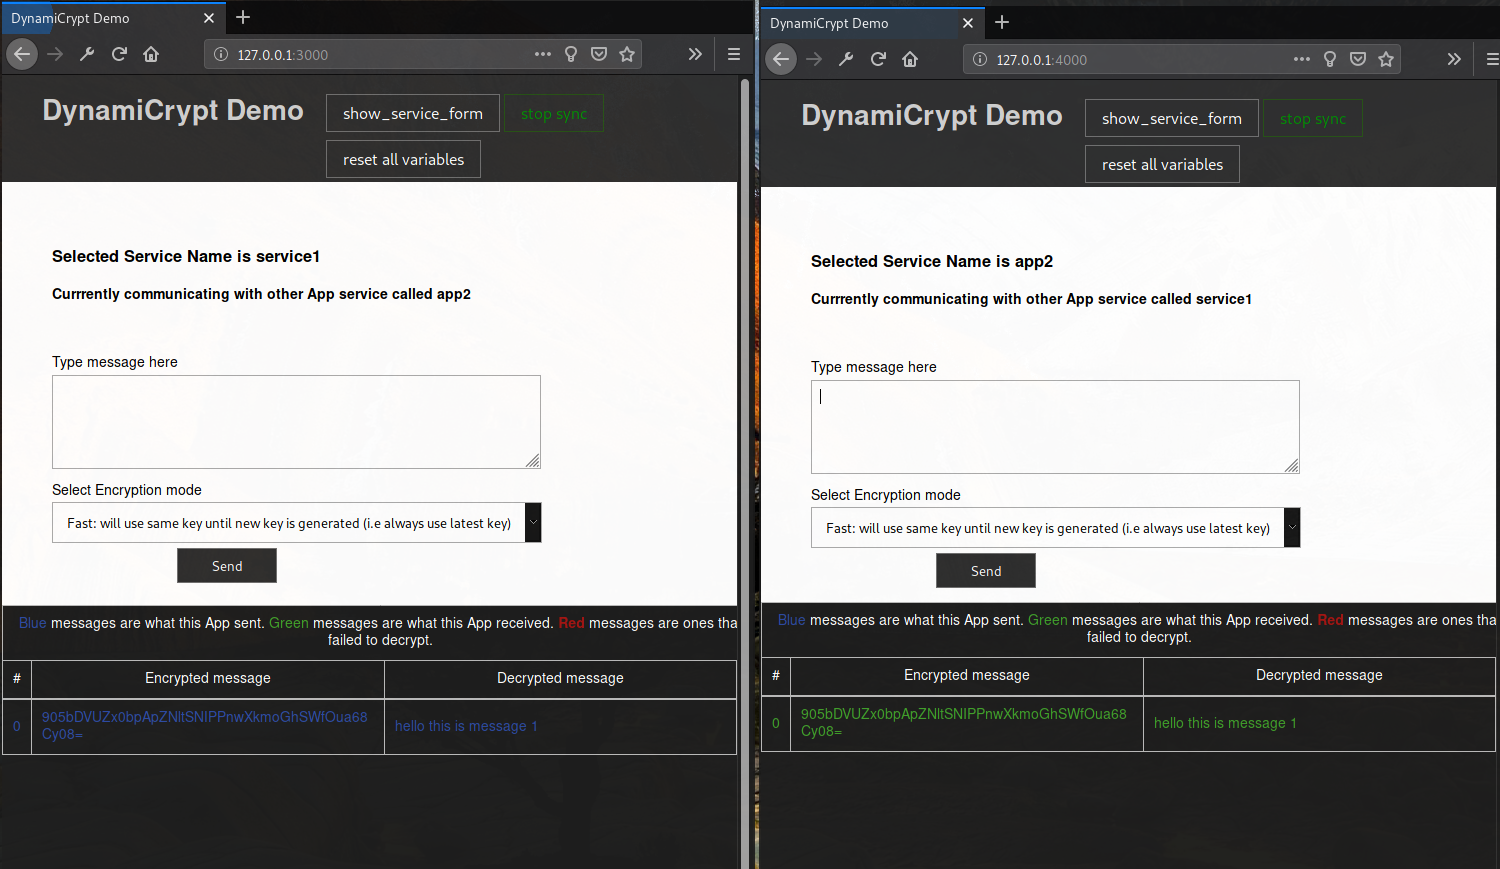
\includegraphics[width=1\textwidth]{Figures/b13.png}
  \caption[Encryption Node App view]{Encryption Node App view}
  \label{fig:b13}
\end{figure}
\FloatBarrier

Figure \ref{fig:b13} shows the two node Apps after a message "hello this is message 1" was sent using the text box interface of the left App. As you can see the right node App decrypted the text successfully.
I will use Wireshark once again to show the data sent between the Node Apps and the API.

\begin{figure}[!h]
  \centering
      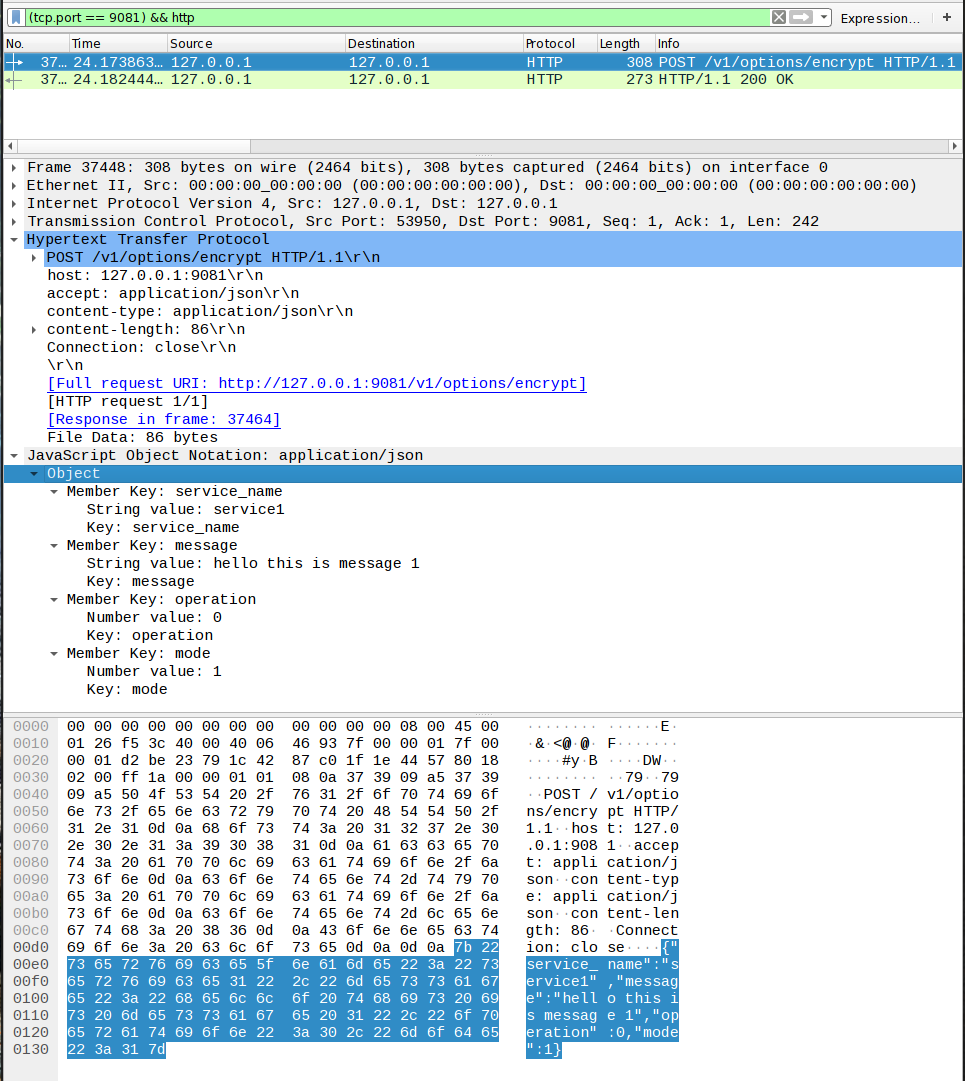
\includegraphics[width=1\textwidth]{Figures/b11.png}
  \caption[Node sends encryption message to the API ]{Node sends encryption message to the API}
  \label{fig:b11}
\end{figure}
\FloatBarrier
Figure \ref{fig:b11} shows the node app at port 3000 sending a post request to the encrypt route of the API.
The data it sends are as follows, service name so the API can identify which key store is appropriate for this service, message the plaintext that will be encrypted, operation this just means whether to encrypt or decrypt because the same route is used, in this case it is 0 but for decryption it would be 1. And finally the encryption mode, mode 1 was chosen in this case.

\begin{figure}[!h]
  \centering
      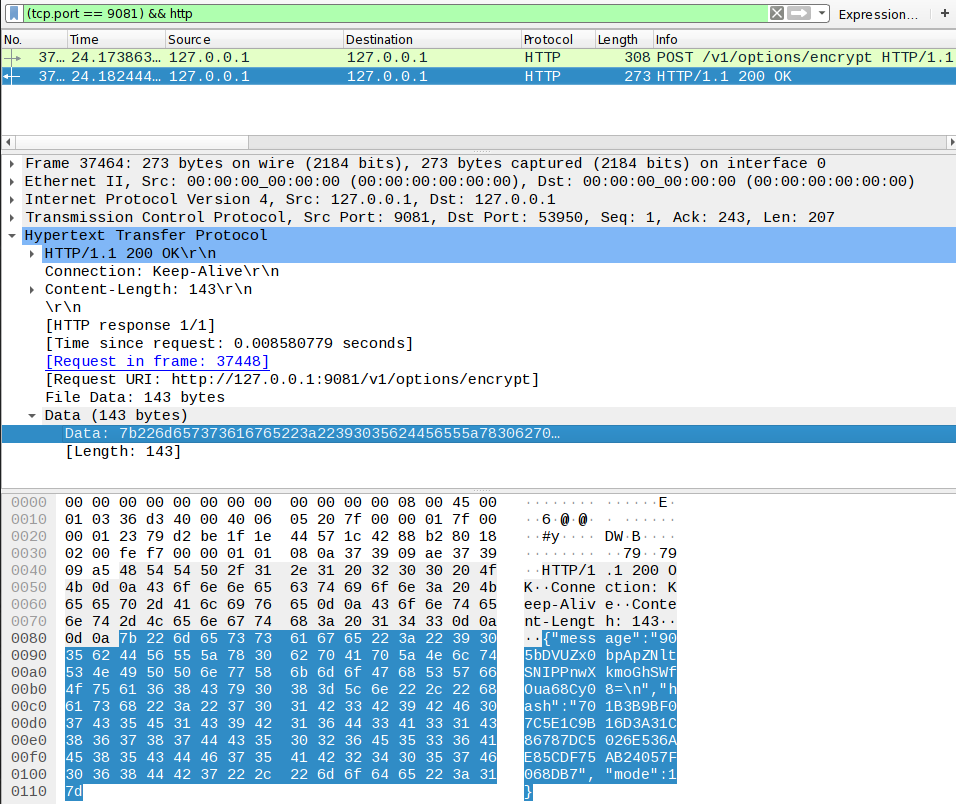
\includegraphics[width=1\textwidth]{Figures/b12.png}
  \caption[API responds with ciphertext and hash]{API responds with ciphertext and hash}
  \label{fig:b12}
\end{figure}
\FloatBarrier
Figure \ref{fig:b12} shows the response of the API, the API replies with the ciphertext as the message, followed by the hash of the plaintext and the mode to be used for decryption. This data will then be forwarded to the other node App by posting it to its decrypt route as seen in figure \ref{fig:b16}


\begin{figure}[!h]
  \centering
      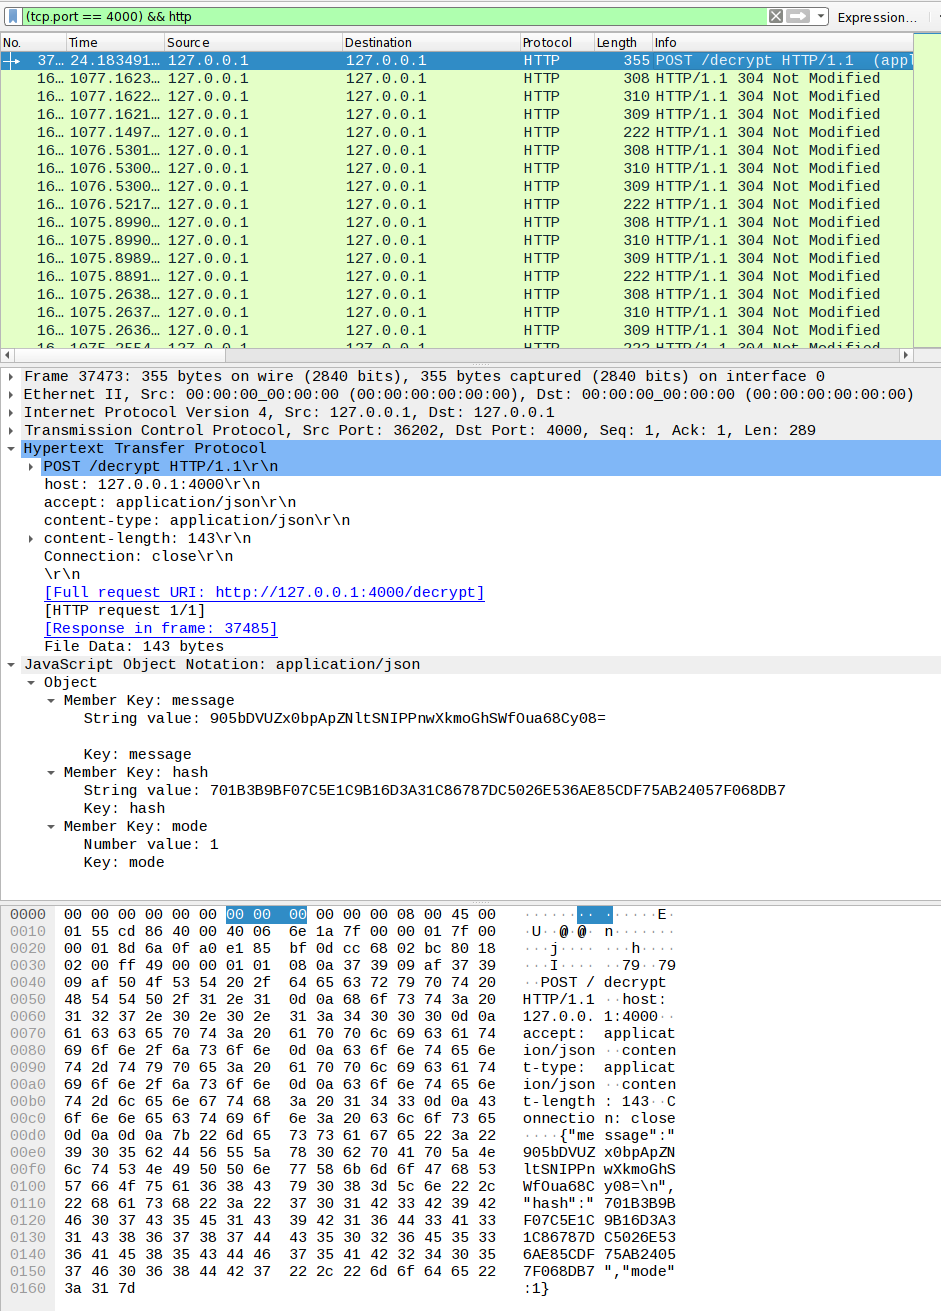
\includegraphics[width=1\textwidth]{Figures/b16.png}
  \caption[Node App at port 3000 sends ciphertext to Node App at port 4000 ]{Node App at port 3000 sends ciphertext to Node App at port 4000 }
  \label{fig:b16}
\end{figure}
\FloatBarrier


\begin{figure}[!h]
  \centering
      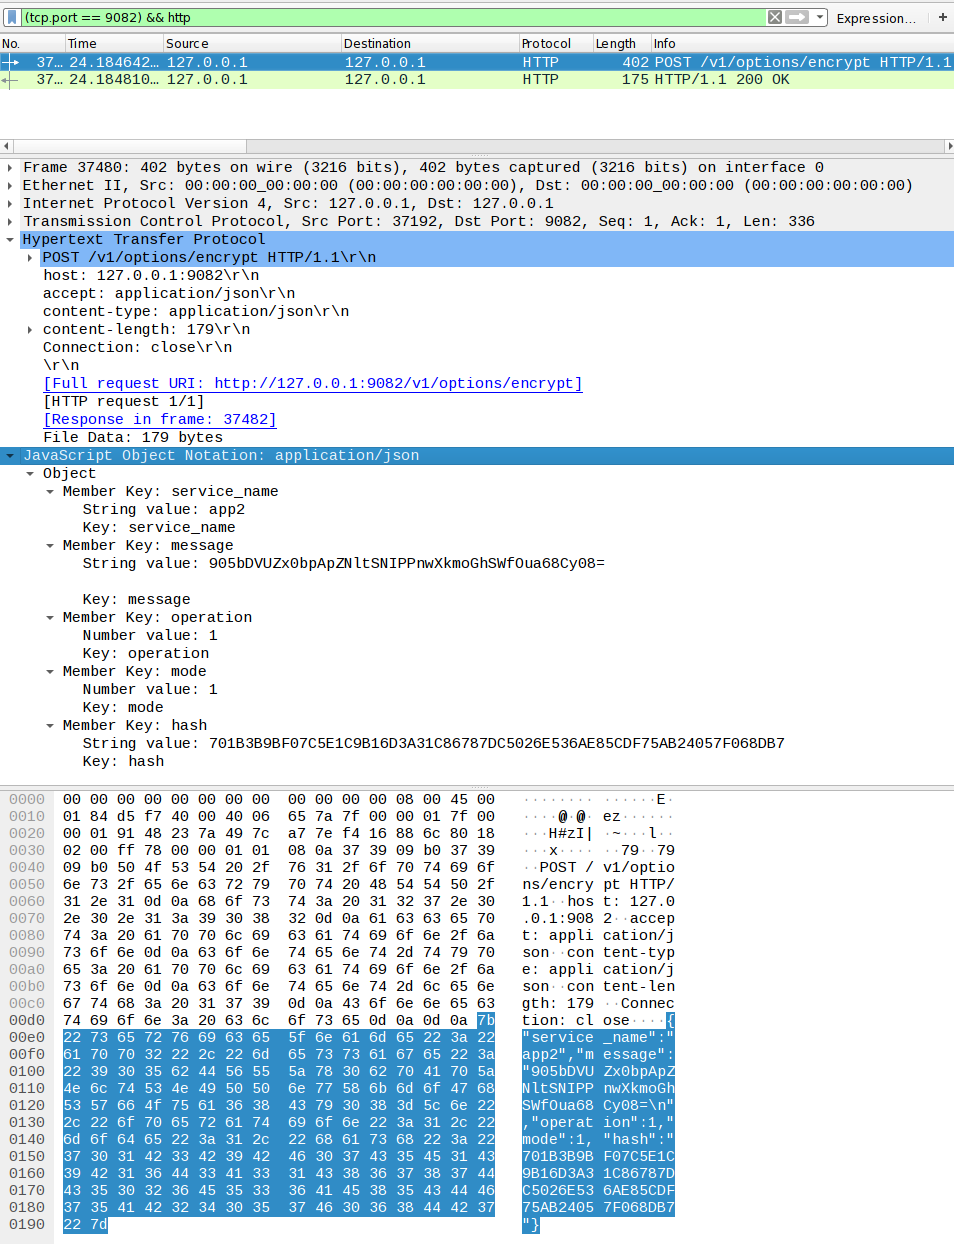
\includegraphics[width=1\textwidth]{Figures/b14.png}
  \caption[Node sends decryption message to the API ]{Node sends decryption message to the API }
  \label{fig:b14}
\end{figure}
\FloatBarrier

Now the node app on port 4000 needs to decrypt the ciphertext so it sends over its service name, ciphertext, operation is 1 this time for decryption, mode is 1 again and finally the hash of the plaintext forwarded from the other API to the API it is using on port 9082. This can all be seen in figure \ref{fig:b14}


\begin{figure}[!h]
  \centering
      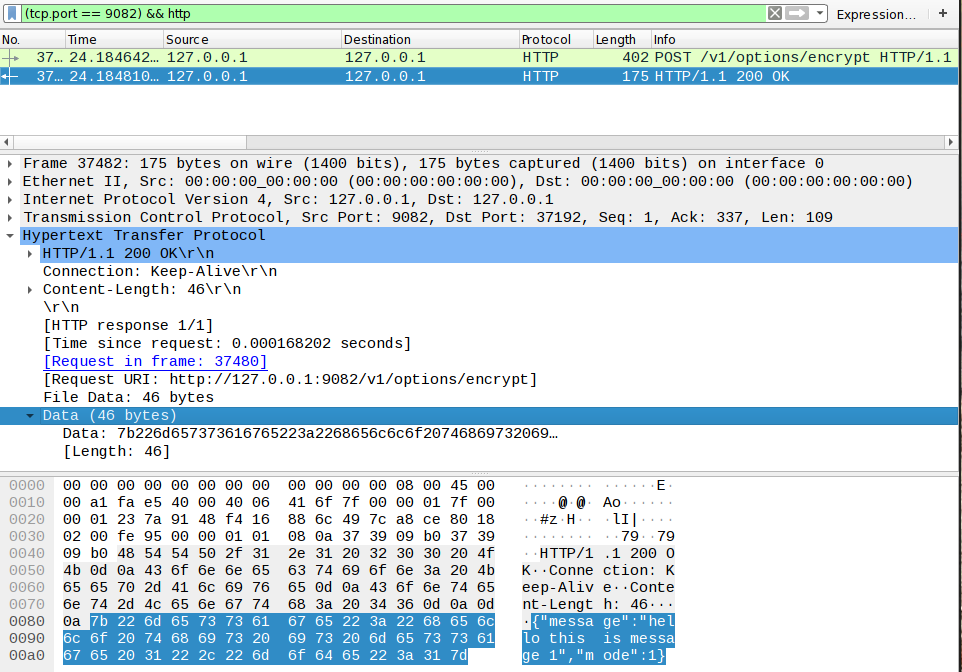
\includegraphics[width=1\textwidth]{Figures/b15.png}
  \caption[API responds with plaintext]{API responds with plaintext}
  \label{fig:b15}
\end{figure}
\FloatBarrier

Figure \ref{fig:b15} is a response from the API, the message was decrypted successfully and is simply sent back to the node app in plaintext the mode is also attached but this is not required for anything other than statistics. 


Next I would like to demonstrate the difference between the encryption modes using the node apps. Basically the point here is that if sending the same message i.e the same plaintext over and over in a non dynamic encryption environment the cipher text that will be produced will always be the same. 
You can see the following demonstration in video form which I mentioned before at this link https://www.youtube.com/watch?v=LsR4XsGrDCY&t=70s

Therefore since this project is all about dynamic encryption the ciphertext will be different every time if using the same plaintext. Note that it is guaranteed to be different every time if mode 2 is used since that will use a unique key for each message, mode 1 on the other hand is built for speed and therefore will use the latest available key therefore if frequent identical plaintexts are sent then there is a possibility that some of the ciphertexts will be the same. 

To test this properly a human would be too slow to type out the message each time so once again I will use a script which will basically submit the form on the browsers behalf. This python script is called send message.py and is once again located inside the GitHub repository.
The script looks like this.
\begin{lstlisting}
#!/usr/bin/env python3.7

import requests
import time

Service_address = "127.0.0.1"
Service_port = 3000

message = "hello -> using mode 1"
encrypt_mode = 1	# 1 for fast. i.e. encrypt using the latest key. 2 for secure only use 1 key once.

how_many_times = 10

url1 = "http://" + Service_address + ":" + str(Service_port) + "/encrypt"
data = {'message':message, 'encrypt_mode': encrypt_mode}

for i in range(0,how_many_times,1):
	print("sending")
	 
	r = requests.post(url = url1, data = data) 
	time.sleep(0.6)
\end{lstlisting}
As you can see this will send the message "hello -> using mode 1" to the encrypt route of the node app on port 3000 ( yes both the node app and the API have an encrypt route, only realised this might be confusing just now ).
This message will be sent 10 times and after each message is sent there will be a break for 0.6 seconds.
Firstly I will use encrypt mode 1.


\begin{figure}[!h]
  \centering
      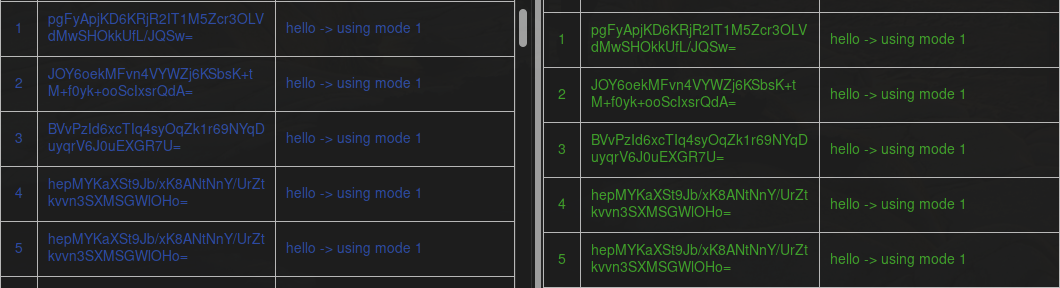
\includegraphics[width=1\textwidth]{Figures/b17.png}
  \caption[Encryption / Decryption mode 1 part 1]{Encryption / Decryption mode 1 part 1}
  \label{fig:b17}
\end{figure}
\FloatBarrier

\begin{figure}[!h]
  \centering
      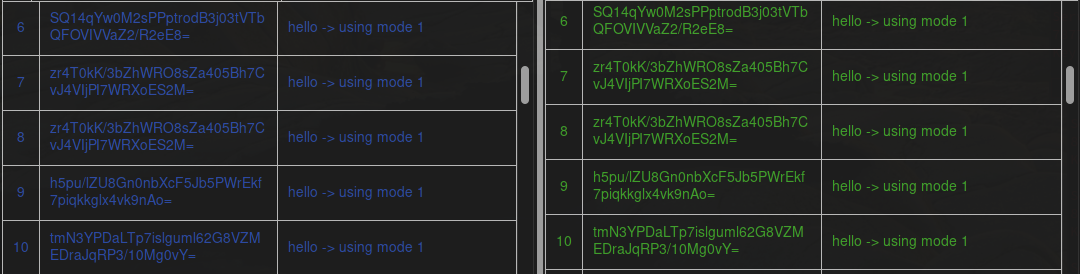
\includegraphics[width=1\textwidth]{Figures/b18.png}
  \caption[Encryption / Decryption mode 1 part 2]{Encryption / Decryption mode 1 part 2}
  \label{fig:b18}
\end{figure}
\FloatBarrier

Figures \ref{fig:b17} and \ref{fig:b18} show the output of the encryption and decryption table in the NodeJs apps after running the script. Here the plaintext is all the same and as you can see on the right node app they have decrypted successfully. The purpose of this test is to examine the cipher text and see which ones if any used the same key.
message 1 used a key unique to itself.
message 2 used a key unique to itself.
message 3 used a key unique to itself.

however message 4 and 5 have the same ciphertext therefore they have used the same key this is because by the time message 5 was encrypted no need key was generated yet and since this is mode 1 it just used the latest key available which happened to be the same one as message 4.

message 6 used a key unique to itself.

message 7 and 8 once again used the same key as each other.

message 9 used a key unique to itself.

message 10 used a key unique to itself.

Given that only two plaintexts were encrypted using the same key twice this is actually a very good result for mode 1. In my previous testing normally you would see three messages in a row encrypted with the same key. This time the keys were generated quicker than expected. How keys are generated will be covered in the sync-server section after this API section. 

Now we will have a look at using mode 2 for encryption to use mode 2 I simply modified two variables in the script.
\begin{lstlisting}
message = "hello -> using mode 2"
encrypt_mode = 2
\end{lstlisting}

\begin{figure}[!h]
  \centering
      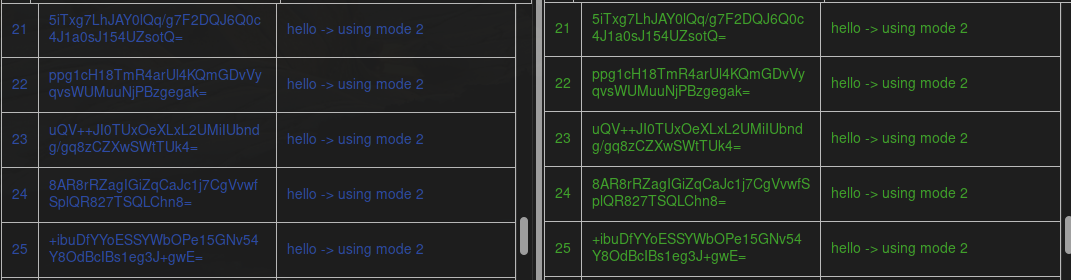
\includegraphics[width=1\textwidth]{Figures/b19.png}
  \caption[Encryption / Decryption mode 2 part 1]{Encryption / Decryption mode 2 part 1}
  \label{fig:b19}
\end{figure}
\FloatBarrier

\begin{figure}[!h]
  \centering
      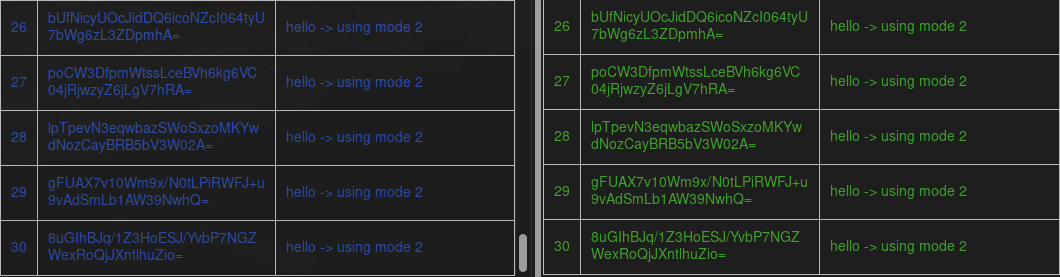
\includegraphics[width=1\textwidth]{Figures/b20.png}
  \caption[Encryption / Decryption mode 2 part 2]{Encryption / Decryption mode 2 part 2}
  \label{fig:b20}
\end{figure}
\FloatBarrier
Figures \ref{fig:b19} and \ref{fig:b20} show the output of the encryption and decryption table in the NodeJs apps after running the script with the modifications.
By looking at the ciphertexts part of the table of the Apps you can see that they are all different despite the same plaintext being used, therefore each message was encrypted using its own unique key and decrypted successfully as can be seen on the right app. 

This means that my algorithm works perfectly for both modes of operation.

As we can see both modes demonstrated dynamic cryptography. Mode 2 is in my opinion is more secure as each message no matter what is encrypted using a unique key. However there is a possibility that you will run out of suitable keys if sending loads of data frequently. If this happens you will just have to wait a little bit for new keys to be generated and encrypt again. 
Mode 1 therefore is perfect if you would like to send loads of data at regular intervals since there will be no issue with running out of keys, you will still reap the benefits of dynamic encryption since it takes around one second or so to generate new keys ( testing time of key generation will be seen later ). 

This will conclude the explanation and testing of aspects related to the API. If I were to explain everything related to the API it would take another 50 pages or so to go through everything therefore I selected the most impact full aspects of the API based on the outcomes of the project and left out most of the technical aspects. This section should have provided a good understanding of most of the more important operations of the API, it is recommended to browse through the GitHub repository for a full exposure of the API. 